\section*{Q3}
Figure 1. illustrates the BLEU scores of rerankers using a variety of feature combinations.

\begin{figure}
	\centering
	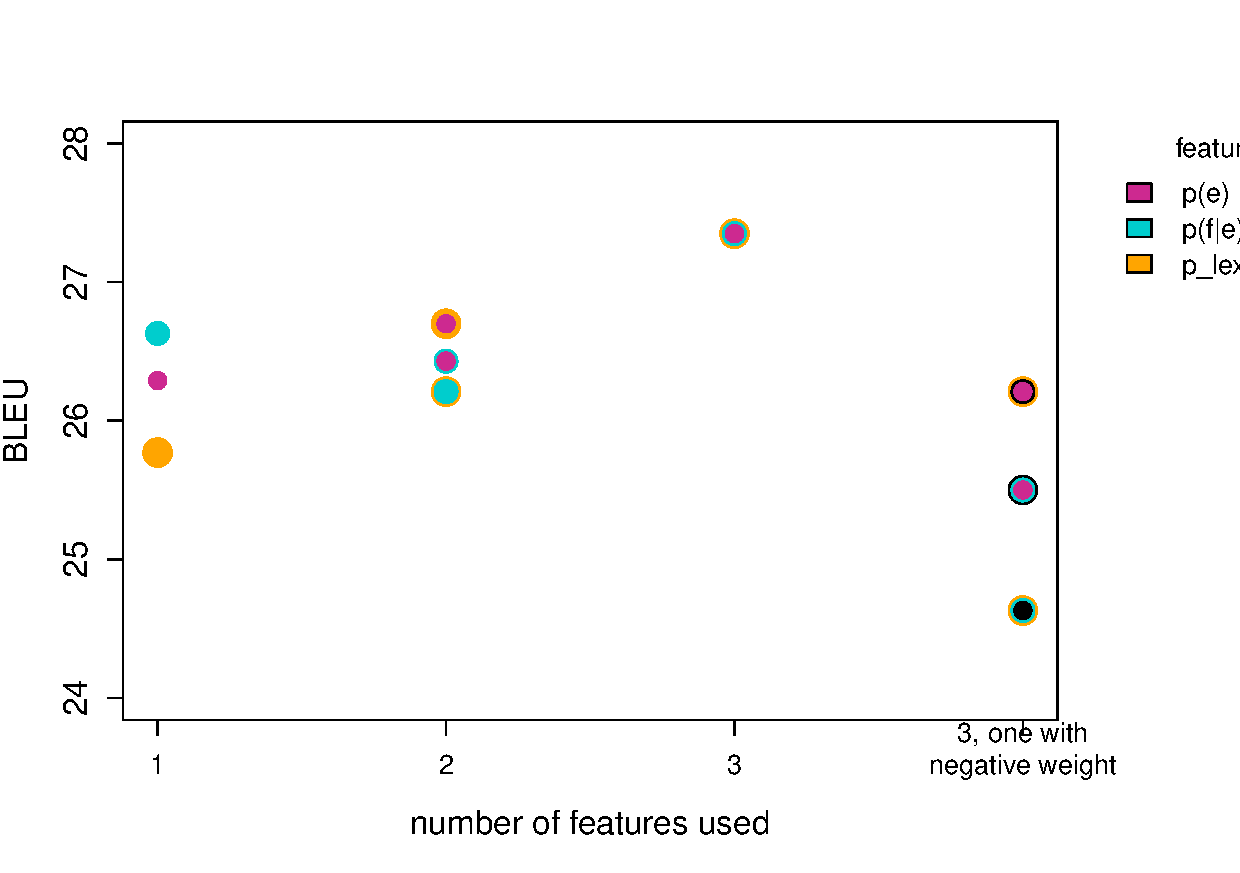
\includegraphics[scale=.65]{figures/q3.pdf}
	\caption{BLEU score as dependent on candidate translation features used for reranking.}
\end{figure}

BLUE score with default feature weights: 27.35
Language model:
	only				  26.29
	without				26.21
	negative		    24.63
	only negative	 24.19
	
Translation model:	
	only				  26.63
	without				26.70
	negative		    26.21
	only negative	 25.58	

Lexicalized reverse translation model
	only				  25.77
	without				26.43
	negative		    25.50
	only negative	 24.84

The first thing to note is that the best BLEU score model is achieved when all three features are used, which suggests that all of them contribute useful information. We can approach the question of relative importance of the features from different angles.

Which feature provides the best performance when used alone?
TM likelihood.

Exclusion of which feature causes the largest performance decrease relative to the default system?
LM likelihood

Reversal of which feature causes the largest performance decrease relative to the default system?
LM likelihood

The influence of particular features on the BLEU score is quite opaque. There is no single most informative feature. Interestingly, combining TM likelihood with one other feature has a negative influence on the score, but combining it with both brings the score to maximum.  
